\documentclass[20pt,margin=0.75in,innermargin=-4.5in,blockverticalspace=-0.35in]{tikzposter}
\geometry{paperwidth=42in,paperheight=30in}
\usepackage[utf8]{inputenc}
\usepackage{amsmath}
\usepackage{amsfonts}
\usepackage{amsthm}
\usepackage{amssymb}
\usepackage{mathrsfs}
\usepackage{graphicx}
\usepackage{adjustbox}
\usepackage{enumitem}
\usepackage{wrapfig,lipsum,booktabs}

\usepackage[backend=biber,style=numeric]{biblatex}
\usepackage{emory-theme}
\DeclareMathOperator{\EX}{\mathbb{E}}% expected value
\usepackage{tabularx}
\usepackage{booktabs}       % professional-quality tables

\usepackage{amsmath, mathtools, amsthm, amssymb}
\usepackage{float}
\usepackage{tabularx}

\usepackage{algorithm}
\usepackage{algorithmic}
\usepackage{pdfpages}


\usepackage[compact]{titlesec}         % you need this package

\usepackage{tabularx}

\usepackage{algorithm}
\usepackage{algorithmic}

\usepackage{graphicx}
\usepackage{subfig}

\usepackage{algorithm}
\usepackage{algorithmic}

\usepackage{mwe} % for placeholder images

\addbibresource{refs.bib}

% set theme parameters
\tikzposterlatexaffectionproofoff
\usetheme{EmoryTheme}
\usecolorstyle{EmoryStyle}

\titlegraphic{
\includegraphics[width=0.03\textwidth]{google-1018443_960_720.png}}
\title{Multi-Environment Pretraining Enables Transfer to Action Limited Datasets}
\author{David Venuto\textsuperscript{$1,2$}, Sherry Yang\textsuperscript{$3,4$}, Pieter Abbeel\textsuperscript{$4$}, Doina Precup\textsuperscript{$1,2,5$}, Igor Mordatch\textsuperscript{$3$}, Ofir Nachum\textsuperscript{$3$}}
\institute{\textsuperscript{$1$}McGill University, \textsuperscript{$2$}Mila, \textsuperscript{$3$}Google Brain, \textsuperscript{$4$}University of California, Berkeley, \textsuperscript{$5$}DeepMind}
\titlegraphic{
\includegraphics[width=0.12\textwidth]{google-1018443_960_720.png}}

% begin document
\begin{document}
\maketitle
\centering
\begin{columns}
    \column{0.32}
    \block{Motivation and Method}{
\begin{itemize}
\item Using massive datasets to train large-scale models has emerged as a dominant approach  for  broad  generalization.
\item Many works have shown that a similar approach can be applied to tasks more often tackled by RL.
\item In RL, available data of sequential decision making is mostly not annotated with actions.
\end{itemize}
\vspace{2mm}

\textbf{Method}
\begin{itemize}
\item Propose combining large but sparsely-annotated datasets from a \emph{target} environment of interest with fully-annotated datasets from other \emph{source} environments.
\item We leverage the generalization capabilities of inverse dynamics modelling (IDM) to label missing action data in the target environment.
\item  Limit our annotated datasets equivalent to only $12$ minutes of gameplay forming a practical, easy to use method.
\end{itemize}

\vspace{4mm}

    }
    \block{Action Limited Pretraining (ALPT)}{
    The dynamics model pretraining procedure of ALPT using the source set of environments along with the limited action target environment dataset.
\begin{tikzfigure}[]
    {{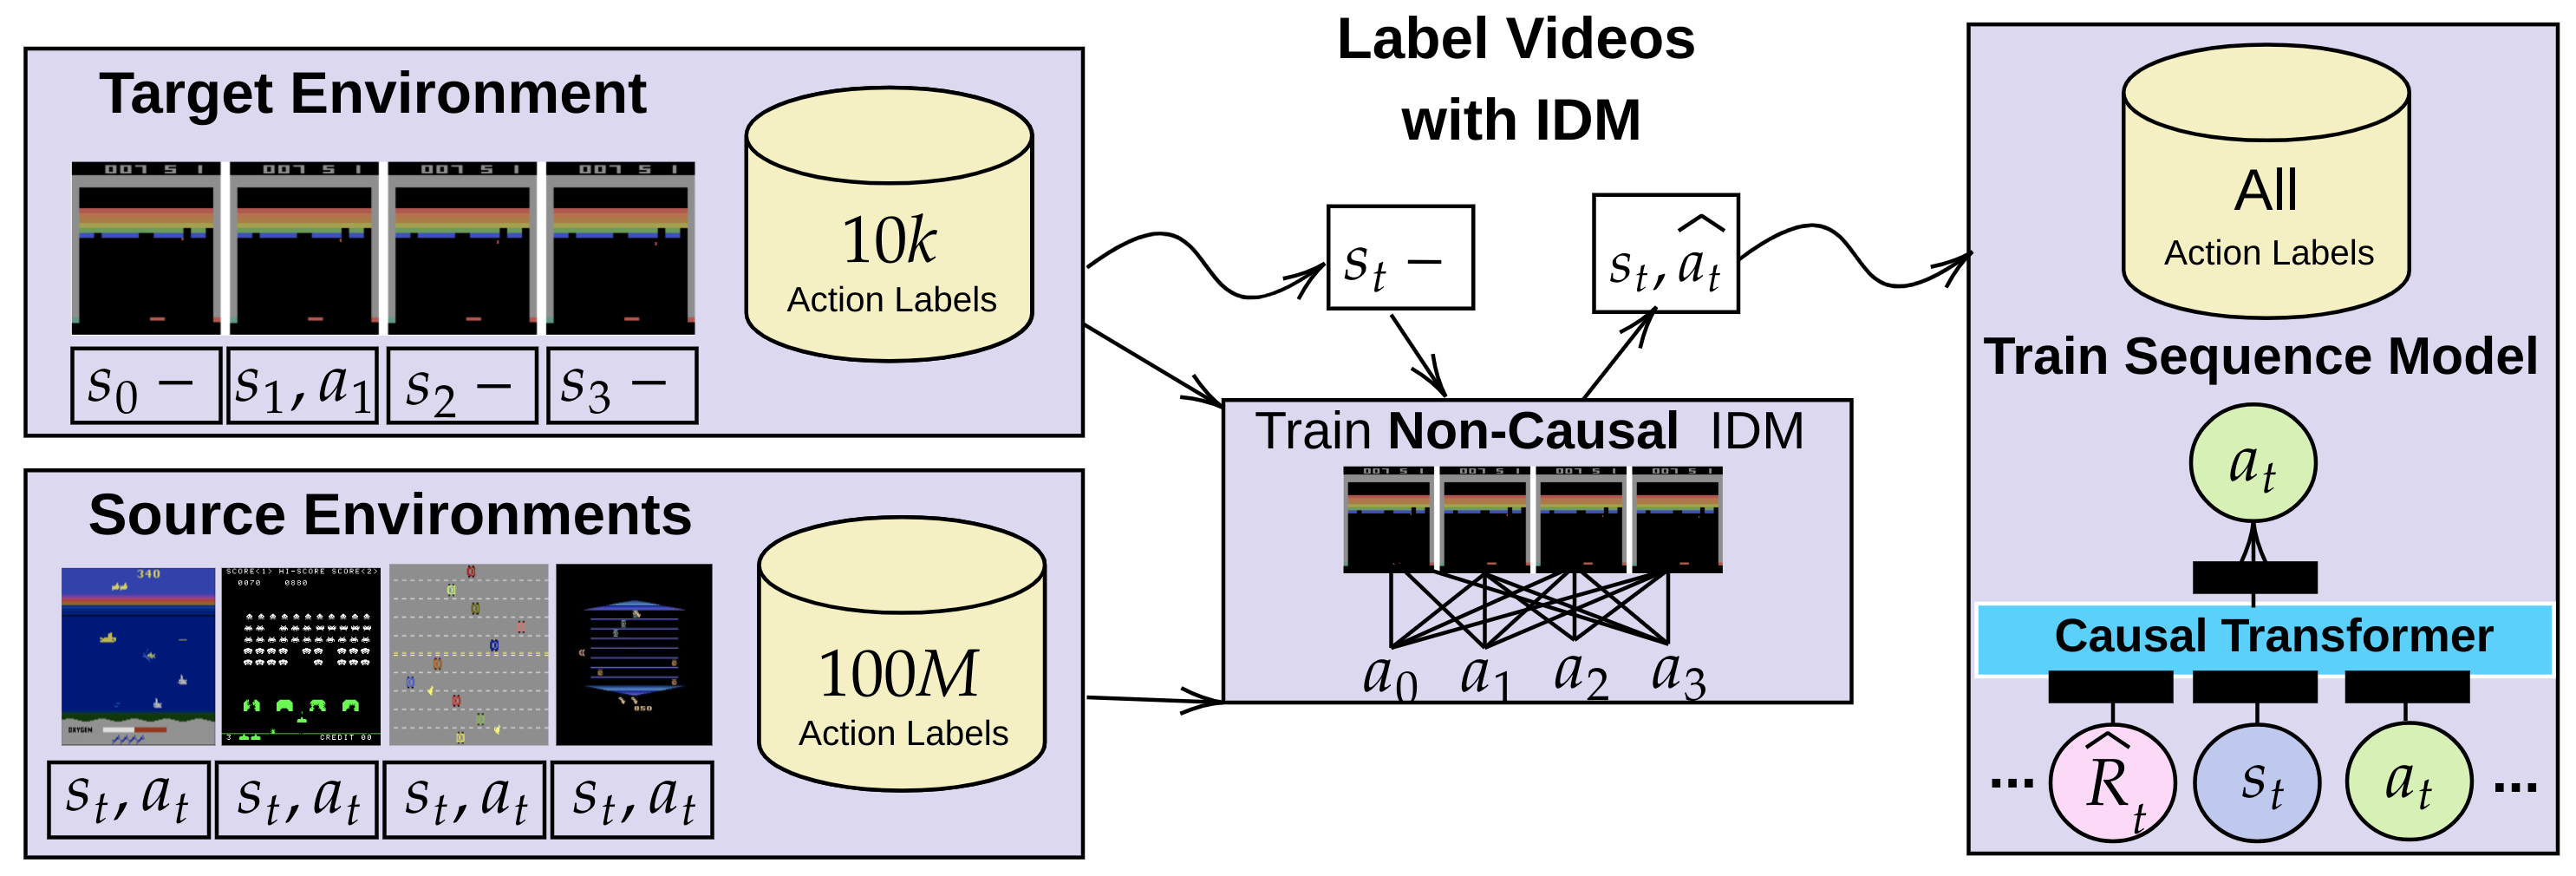
\includegraphics[width=29.5cm]{idm_model.png}}}\hfil%
        \end{tikzfigure}
\vspace{4mm}
}

    \block{Decision Transformer}{
    \begin{itemize}
    \item Decision transformer (DT) is an offline RL approach which formulates the problem as sequence modeling.
    
    \item DT proposes a transformer-based architectures to model the sequence. The tokenized sequence episodes are augmented with the returns at each step:
    \begin{equation}
    \tau = \langle \dots, \mathbf{s_t}, a_t, r_t, G_t,  \dots \rangle.
\end{equation}
\item Utilize causal transformer $P_\theta$, which predicts both returns and actions using a cross-entropy loss.  The learning objective for ${\theta}$ is:
\end{itemize}
\begin{equation}
\label{dtloss}
    J(\theta) = \mathbb{E}_{\tau} \left[\sum_{t} -\log P_\theta(G_t | \mathbf{s}_{\le t},a_{<t},r_{<t}) - \log P_\theta(a_t | \mathbf{s}_{\le t},a_{<t},r_{<t},G_{t}) \right].    
\end{equation}
\vspace{4mm}

    }
    \column{0.34}

\block{Inverse Dynamics Modelling}{
Inverse dynamics models (IDM) use a bidirectional transformer trained to predict actions from an action-unlabelled sub-trajectory. The training objective for learning an IDM $P_{\beta}$ is:
\begin{equation}
\label{eq:idm}
    J(\beta) = \E_{\tau}\left[\sum_t \sum_{i=0}^{k-1} - \log P_{\beta} (a_{t+i} | \mathbf{s}_t, \dots, \mathbf{s}_{t+k})\right],
\end{equation}
where $k=5$ is the length of training sub-trajectories.
\vspace{4mm}

}

\block{Multi-Environment Training and Finetuning}{
\vspace{-3mm}
\begin{itemize}
\item We have $n$ \emph{source} environments, defined by MDPs: $E =\{\mathcal{M}_1,\dots,\mathcal{M}_{n_{}}\}$, and a single \emph{target} environment $\mathcal{M}_\star$. 
\item For each $\mathcal{M}_d$, the agent can access a dataset of episodes from $\mathcal{M}_d$, denoted by $\mathcal{D}_d = \left\{\tau:=\langle \dots,\mathbf{s}_t, a_t, r_t, \dots \rangle\right\}$, \textbf{fully labelled with actions}.  
\item For the \emph{target environment}, the agent can access to a \textbf{small labelled dataset} from $\mathcal{M}_\star$, denoted as $\mathcal{D}^+_\star = \left\{\tau:=\langle \dots,\mathbf{s}_t, a_t, r_t, \dots \rangle \right\}$, and a \textbf{large dataset without action labels}, $\mathcal{D}^-_\star = \left\{\tau:=\langle \dots,\mathbf{s}_t, r_t, \dots \rangle \right\}$.  %We denote the combined action limited dataset of the target environment as $\mathcal{D}_\star = \mathcal{D}^-_\star \cup \mathcal{D}^+_\star $.
\end{itemize}
The \textbf{Pretraining and Finetuning} procedure is summarized below:
\vspace{4mm}
\begin{tabular}{ll}
\multicolumn{1}{c}{\bf Step} & 
\multicolumn{1}{c}{\bf Procedure} 
\\ \hline \\
\textbf{Pretraining} & Train IDM on all labelled data: $\left(\bigcup_{d=1}^n \mathcal{D}_d\right)\cup\mathcal{D}^+_\star$. \\
& Train DT on all data: $\left(\bigcup_{d=1}^n \mathcal{D}_d\right)\cup\mathcal{D}^+_\star\cup\mathcal{D}^-_\star$, with IDM \\
& providing action labels on $\mathcal{D}^-_\star$ 
\\ \hline \\
\textbf{Finetuning}             & 
Train IDM on labelled data in target environment dataset: $\mathcal{D}^+_\star$. \\ 
& Train DT on all data in target environment dataset: $\mathcal{D}^+_\star\cup\mathcal{D}^-_\star$, \\
& with IDM providing action labels on $\mathcal{D}^-_\star$ 
\\ \hline \\
\textbf{Evaluation}             & 
Use trained DT agent to interact with target environment $\mathcal{M}_\star$. \\
\end{tabular}
\vspace{4mm}

}

\block{Experiments}{
\textbf{Single-game variants.} We evaluate the benefit of multi-game versus single-environment training. 

\begin{itemize} \item \textbf{DT1}: we train a DT only on the $10$k subset of data that is labelled, 
\item \textbf{DT1-IDM}: we train DT and IDM simultaneously  we use the IDM to provide action labels on the unlabelled portion of the data. 
\end{itemize}
\textbf{Multi-game DT variants.} We assess the need for IDM versus training on DT with multiple games alone.
\begin{itemize} \item \textbf{DT5}: We evaluate a multi-game baseline composed of DT alone. We pretrain DT on all labelled datasets combined from both the source and target environments before finetuning the DT model on the $10k$ labelled portion of the target game. %We pretrain a DT on all games from the limited set of Atari games and evaluate it on a single selected game.  The IDM is used to label the missing actions on the target game.  This training dataset contains all true action labels from the source set of non-evaluation games and only a limited amount of labeled actions ($10K$) on the evaluation game.  We pretrain a DT \textbf{with} and \textbf{without} IDM labelling, denoted as \textbf{ALPT} (our method) and \textbf{DT5} respectively.
\item \textbf{DT5-RET}: we uses the unlabelled portion for training its return prediction.
\end{itemize}

}
    \column{0.34}

\block{How Does ALPT Compare to Baselines?}{
 Target game performance during finetuning on the limited action target dataset.  
\begin{tikzfigure}[]%
\begin{center}
\subfloat{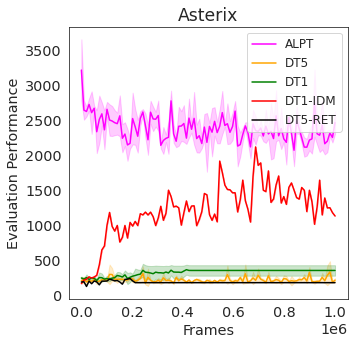
\includegraphics[width = 4in]{asterix.png}} 
\subfloat{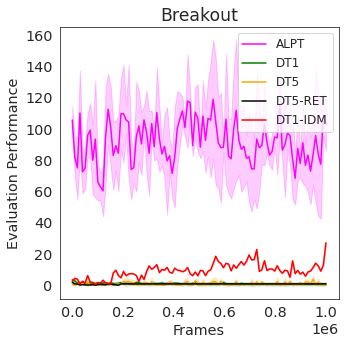
\includegraphics[width = 4in]{breakout.png}}
\subfloat{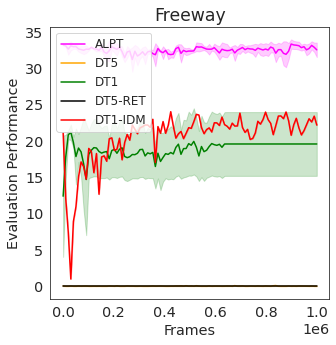
\includegraphics[width = 4in]{freeway.png}} \\
\centering
\subfloat{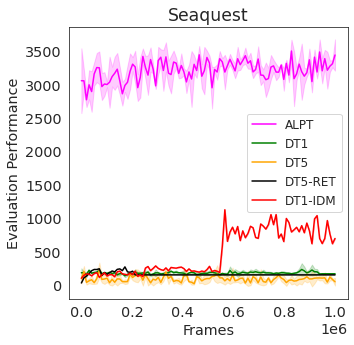
\includegraphics[width = 4in]{seaquest.png}} 
\subfloat{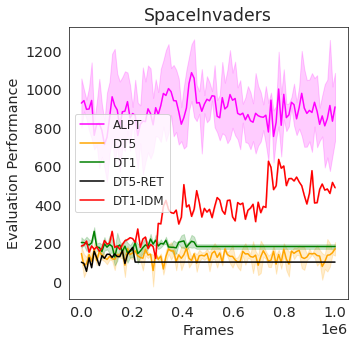
\includegraphics[width = 4in]{spaceinvaders.png}}  \hspace{0.0cm}%
        \end{center}
\end{tikzfigure}
}
\block{Disjoint Action Spaces Experiments}{
\begin{itemize}
\item  Explore pretraining on source environments where the action space ($\mathcal{A}_d$) is disjoint with the target environment action space ($\mathcal{A}_*$), that is, $\mathcal{A}_d \cap \mathcal{A}_* = \emptyset$. \item Example: \emph{Freeway} with \{Up, Down\} and \emph{Breakout} with \{Left, Right\}. 
\end{itemize}
        \vspace{-6mm}
\begin{tikzfigure}[]%
\subfigure{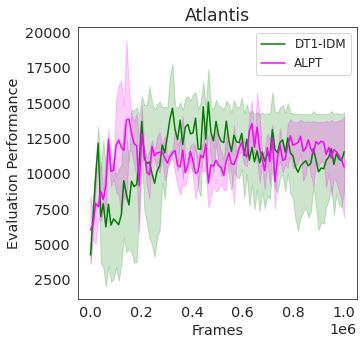
\includegraphics[width = 3.0in]{atlantis_disjoint.png}} 
\subfigure{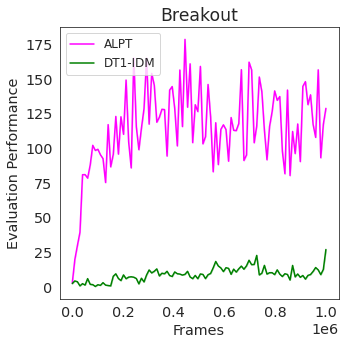
\includegraphics[width = 3.0in]{breakout_disjoint.png}}
\subfigure{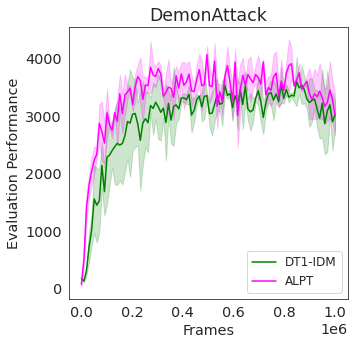
\includegraphics[width = 3.0in]{demon_attack_disjoint.png}} 
\centering
\subfigure{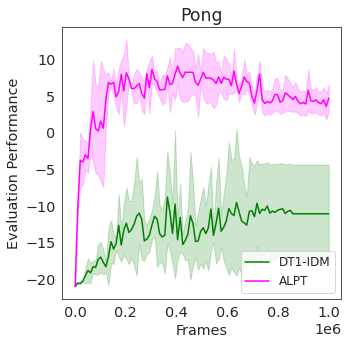
\includegraphics[width = 3.0in]{pong_disjoint.png}}\\ 
\subfigure{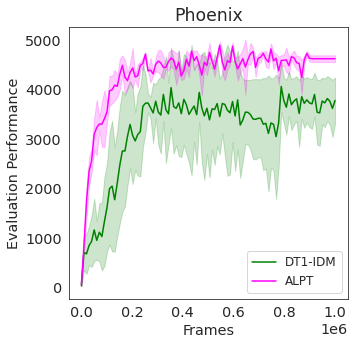
\includegraphics[width = 3.0in]{phoenix_disjoint.png}} 
\subfigure{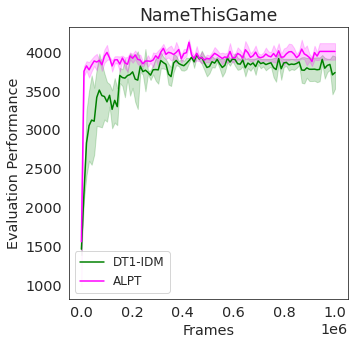
\includegraphics[width = 3.0in]{name_this_game_disjoint.png}}  
\subfigure{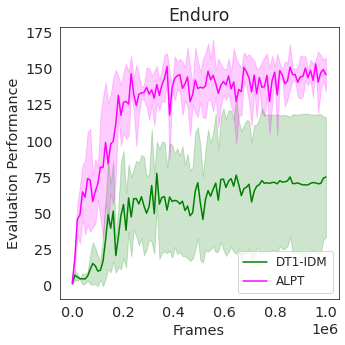
\includegraphics[width = 3.0in]{enduro_disjoint.png}}
\subfigure{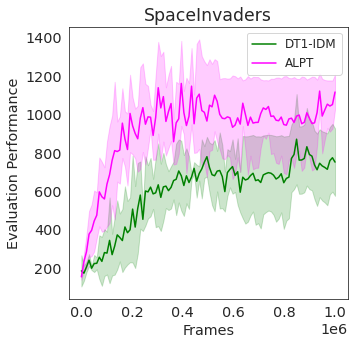
\includegraphics[width = 3.0in]{space_invaders_disjoint.png}} 
\end{tikzfigure}
}

\block{Conclusion}{
\vspace{-2mm}
\begin{itemize}
    \item  Our results  support the importance of generalist inverse dynamics models as an efficient way to implement large-scale RL.
\item As more labelled data becomes available, ALPT provides an efficient way of bootstrapping performance on new tasks with action limited data.
\end{itemize}

}


\end{columns}
\end{document}